This section discusses the rules and implementation details of Baba is AI, the task
environment used in experiments in Section 4. Baba is AI is derived from Baba is
You, a grid-based puzzle video game, and was originally implemented as part of the
BALROG \cite{paglieri2024balrog} agent benchmark.

Baba Is You is a puzzle game where the player controls a character that can navigate
and modify the rules of the game by pushing blocks containing words such as 'you',
'is' 'key', that, when combined, define the game's rules.

The game field consists of a rectangular 4-connected grid with a number of objects,
rules blocks, and obstacles present.

\begin{figure}[ht]
	\centering
	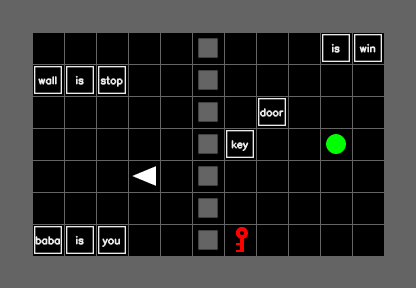
\includegraphics[scale=0.75]{figs/babaisai_env.png}
	\caption{Example of the baba-is-ai environment. In this task (\textit{two\_room-break\_stop-make\_win-distr\_obj-irrelevant\_rule}),
	the agent has to break the "wall is stop" rule by pushing either 'wall', 'is',
	or 'stop' out of alignment with the other blocks, and must then push the "key"
	rule block next to "is win" at (9, 1) to assemble the win rule, then touch the
	key at (7, 7) to win. Pushing the "door" rule block would be a mistake, as no door
	object is present.}
	\label{fig:babaisai_env}
\end{figure}

Words (represented as rule blocks) can be combined to form sentences that define
the properties of objects, rules, and obstacles in the game, with rules becoming
active when a full sequence of rule blocks are joined in a 3-block line horizontally
or vertically.

Active rules are built in the form [<subject> <verb> <object>], where the
subject and object are the names of objects in the game, and the verb is one of the
following: "is", "has", "can", or "not".

The goal of the game is to reach a win condition, by manipulating the rules of
the game to create new win conditions, modify the properties of objects, or
change the behavior or identity of the player character.

The testing implementation we use is the baba-is-ai environment, a simplified version
of Baba is You originally implemented within the BALROG agent benchmark \cite{cloos2024babaaibreakrules,
paglieri2024balrog}. This implementation has several simplifications compared to
the original game, including a smaller grid size, fewer objects, and a limited set
of rules. The environment is designed to be easy to use and understand, while still
providing a challenging testbed for evaluating the performance of reinforcement learning
agents on agentic reasoning tasks.

A single baba-is-ai task is defined by an arbitrary rectangular grid where an exit
condition must be reached, with several possible obstacles and rules preventing
the player from reaching the exit. Intermediate goals to achieving the exit condition
can be defined by the user, and the environment will generate a task that
requires the agent to learn how to manipulate the rules of the game in order to
reach the exit. These intermediate goals are referred to as "subtasks" within our
paper, and include:

\begin{itemize}
	\item \textbf{Goto-Win}: The agent must reach a specific location on the grid.

	\item \textbf{Make-Win}: The agent must create a new win condition by manipulating
		the rules of the game.

	\item \textbf{Break-Stop}: The agent must break or bypass a wall or obstacle in
		order to reach the exit.

	\item \textbf{Change-You}: The agent must change the identity of the player character
		in order to reach the exit, by modifying the "baba is you" rule.
\end{itemize}

These subtasks can be arbitrarily combined with distractor objects or rules,
immovable game field walls, and each other to generate tasks of varying complexity
and length; baba-is-ai implements 40 total unique tasks of gradually increasing
difficulty.

The agent is provided observations in a text form, which includes the current state
of the game field, the currently active rules, and relative locations of obstacles
to the active player character in terms of shortest Manhattan distance. This is
done to make the environment compatible with purely text-based language models.

The agent is provided the space of possible actions it can take, which consist moving
one space in one of the four cardinal directions (up, down, left, right), but is
not given information about whether a given move will result in movement; it is
thus free to move into immovable walls without effect, to push rule blocks into corners
where they cannot be moved, or to make the task unsolvable by breaking the
active "baba is you" rule without taking control of a new object; in this last instance,
the environment automatically resets the task to a randomized beginning state
for that task.

The environment is limited to 100 steps per task episode to avoid tasks being
solved by random walks.